\documentclass[12pt]{article}
\usepackage{amssymb,amsmath,natbib,graphicx,amsthm,
  setspace,sectsty,anysize,dsfont,enumerate}

\usepackage{times}

\usepackage[svgnames]{xcolor}

\usepackage{lscape,arydshln,relsize,rotating}
\usepackage[small]{caption}
\usepackage{algorithm}

\graphicspath{{/home/taddy/project/distributed_multinomial_regression/graphs/}}

\newtheorem{prop}{\sc Proposition}[section]
\renewcommand{\qedsymbol}{}

\marginsize{1.1in}{.9in}{.3in}{1.4in}

\newcommand{\nb}{\color{blue}}
\newcommand{\dbl}{\setstretch{1.5}}
\newcommand{\sgl}{\setstretch{1.1}}

\newcommand{\bs}[1]{\boldsymbol{#1}}
\newcommand{\mc}[1]{\mathcal{#1}}
\newcommand{\mr}[1]{\mathrm{#1}}
\newcommand{\bm}[1]{\mathbf{#1}}
\newcommand{\ds}[1]{\mathds{#1}}
\newcommand{\indep}{\perp\!\!\!\perp}
\DeclareMathOperator*{\argmin}{argmin}
\newcommand{\norm}[1]{|\!|#1|\!|_{1}}
\newcommand{\cd}[1]{{\tt#1}}
\newcommand{\e}[1]{{\footnotesize$\times10$}{$^{#1}$}}

\sectionfont{\noindent\normalfont\large\bf}
\subsectionfont{\noindent\normalfont\normalsize\bf}
\subsubsectionfont{\noindent\normalfont\it}

\usepackage[bottom,hang,flushmargin]{footmisc}

\pdfminorversion=4
\begin{document}

\sgl 

\pagestyle{empty}

~
\vskip 3cm

\noindent {\huge \bf Distributed Multinomial Regression} 

\vskip 1cm

\noindent{\Large Matt Taddy}

{\large
\vskip .5cm \noindent
{The  University of Chicago Booth School of Business}\\
{\tt faculty.chicagobooth.edu/matt.taddy}}



\vskip 2cm

{\noindent This article introduces a model-based approach to distributed
computing for multinomial logistic regression. We treat
counts for each response category as independent Poisson regressions
via plug-in estimates for fixed effects shared across categories.  The work is
driven by the high-dimensional-response multinomial models that
arise in analysis of a large number of random counts. Our archetypal
applications are in text analysis, where documents are tokenized
and the token counts are modeled as arising from a  multinomial dependent upon
document attributes. We estimate such models for a publicly available dataset
of reviews from Yelp, with text regressed onto a
large set of explanatory variables (user, business, and rating information).
The fitted models serve as a basis for exploring the connection between
words and variables of interest (e.g., star rating), for reducing dimension
into supervised factor scores, and for prediction. }
 

\newpage
\dbl

\pagestyle{plain}
\vskip 1cm
\section{Introduction}
\label{intro}


This article is motivated by datasets that include {\it counts} in a massive
number of {\it categories}, such as text corpora (counts for words), browser
logs (counts on websites), and website tracking (counts of clicks). The unit
upon which counts are observed -- e.g., a `document' for text or a `user' in
web analysis -- is annotated with {\it attributes}, additional information
about each document (author, date, etc) or user (age, purchases, etc).  Much
of contemporary Big data analysis involves some exploration, inference, and
prediction of, or controlling for, the relationship between these attributes
and the associated very-high-dimensional counts.


Say $\bm{c}_i$ is a vector of counts in $d$ categories, summing to $m_i =
\sum_j c_{ij}$, accompanied by a $p$-dimensional attribute vector $\bm{v}_i$ on observation
unit $i$ of $n$ total.  For example, in the archetypal text mining application, $\bm{c}_i$
are counts for words in document $i$ annotated with metadata $\bm{v}_i$.   We
connect attributes and counts through a big multinomial logistic regression
model,
\begin{equation}\label{bigmn}
\mr{p}(\bm{c}_{i} | \bm{v}_i,m_i) = 
\mr{MN}\left(\bm{c}_i;~\bs{\lambda}_{i}/\Lambda_i,
~m_i\right),~~\text{where}~~\lambda_{ij} = \exp[\alpha_j + \bm{v}_i'\bs{\varphi}_j]~~\text{and}~~\Lambda_i = \sum_{j=1}^d\lambda_{ij}.
 \end{equation} 
 The multinomial denoted $\mr{MN}$ here has, for unit $i$, category $j$ probability
$\lambda_{ij}/\Lambda_i$ and size $m_i$. This model can be computationally
expensive to estimate for a large number of response categories (i.e., big
$\bm{c}_i$ dimension $d$).  Even a single likelihood evaluation is costly, due
to the sum required for each normalizing {\it intensity} $\Lambda_i$. The
methodological innovation of the current article is to replace $\Lambda_i$
with initial estimates, then condition upon these plug-ins when estimating
(\ref{bigmn}) through $d$ individual Poisson regressions for counts in each
category $j$. This model-based factorization allows one to {\it partition}
computation across many independent machines, so with enough processors the
system of (\ref{bigmn}) is fit in the time required for a single Poisson
regression.

We refer to this framework as {\it distributed multinomial regression}, or DMR.
Our work here extends ideas from \cite{taddy_multinomial_2013}, which
introduced the strategy of {\it multinomial inverse regression} (MNIR).  That
article argues for estimation of models like (\ref{bigmn}) as the first step
in an inverse regression routine for predicting elements of new $\bm{v}_i$.
However, \cite{taddy_multinomial_2013} relies upon a fitting algorithm that
collapses response counts across equal $\bm{v}_i$, and hence scales {\it only}
for a small number of attributes (i.e., when $p$ is just one or two). That
article is also focused exclusively on applications in attribute prediction.
The purpose of the current article is thus two-fold: to supply techniques for
estimation when both $\bm{c}$ and $\bm{v}$ are high dimensional, and to
illustrate how these models can be useful in many aspects of analysis and
inference.

Much of the paper is devoted to an example analysis of reviews on Yelp -- an
Internet platform for feedback on various establishments, including
restaurants, barbers, schools and much else.  This dataset has a rich feature
set associated with a wide variety of reviews. The data are also publicly
available, after (free) registration on the data mining contest website
\cd{kaggle.com}. 
Moreover, our technology is provided in the \cd{distrom} package for R and
 Yelp analysis code is cataloged at \cd{github.com/mataddy/yelp}.  Public
access is essential here: our goal is to provide a
complete template for analysis of high-dimensional count data.

The estimation strategy is detailed in Section \ref{methods}, including model
factorization, plug-ins for $\Lambda_i$, and regularization
path estimation within each parallel regression. Methods
are illustrated in the short classification example of Section
\ref{FGL}, which shows utility for DMR not only in
big $d$ but also as a speedup for small $d$ multinomial regressions. Finally,
Section \ref{YELP} runs through our full Yelp example, detailing model
estimation and a variety of analysis applications.
\begin{itemize}\sgl
\item 
Exploration: what words are associated with funny or useful content?
\item Dimension reduction: which reviews have the most funny or useful content?
\item Prediction: what will be the usefulness or hilarity of a new review? 
\item Inference: does user experience lead to higher star ratings?
\end{itemize}
All of this is built upon {\it partial effects}:  connections
between text and attributes that arise  after controlling for
collinearity between attributes.  Section \ref{END} closes with a short
discussion.


\section{Methods: Estimation in Distribution}
\label{methods}

For convenience, we'll adopt terminology from text analysis for the remainder
and refer to each unit $i$ as a `document' and each category $j$ as a
`word'.\footnote{Even in text mining this is a simplification; each $j$ could
be a combination of words or any other language token.} Suppose that every
document-word count $c_{ij}$ has been drawn independently
$\mr{Po}\left(\lambda_{ij}\right)$ -- Poisson with intensity (i.e., mean)
$\lambda_{ij}$. The joint document likelihood, for $\bm{c}_i$, then factorizes as the
product of a multinomial distribution for  individual counts conditional on
 total count $m_i$ and a Poisson distribution $m_i$.
That is, the multinomial is `embedded' in the Poisson as
\begin{equation}\label{embed} \mr{p}(\bm{c}_{i}) = \prod_j
\mr{Po}\left(c_{ij};~\lambda_{ij}\right) =
\mr{MN}\left(\bm{c}_i;~\bs{\lambda}_{i}/\Lambda_i,
~m_i\right)\mr{Po}\left(m_i;~\Lambda_i\right). 
\end{equation}

This well known result has long been used by statisticians to justify ignoring
whether sampling was conditional on margin totals in analysis of contingency
tables. \cite{birch_maximum_1963} showed that the maximum likelihood estimate
(MLE) of $\bs{\lambda}_i$ is unchanged under a variety of sampling models for
3-way tables {\it under the constraint} that $\Lambda_{i} = m_i$. This is
satisfied at the MLE for a saturated model. \cite{palmgren_fisher_1981}
extends the theory to log-linear regression with $\lambda_{ij} = \exp[\alpha_j
+ \mu_i + \bs{\varphi}_j'\bm{v}_i]$, showing that the Fisher information on
  regression coefficients is the same regardless of whether or not you've
  conditioned on $m_i$  so long as $\mu_i$ in the Poisson model is estimated
  at its conditional MLE, 
 \begin{equation} \label{mlemu}
  \mu_i^\star =
\log\left(\frac{m_i}{\sum_j e^{\alpha_j + \bm{v}_i'\bs{\varphi}_j}}\right).  
\end{equation}

Most commonly, (\ref{embed}) is invoked when applying multinomial logistic
regression: totals $m_i$ are then ancillary and the $\mu_i$ drop out of the
likelihood.  Our DMR framework takes the opposite view: if we are willing to
fix estimates $\hat\mu_i$ potentially not at their MLE (we will argue for
$\hat\mu_i = \log m_i$), then the factorized Poisson likelihood can be
analyzed independently across response categories.\footnote{In an older version
of this idea, \cite{hodges_poisson_1960} introduce a Poisson approximation
to the binomial distribution, for which
\cite{mcdonald_poisson_1980} provides error bounds and extension to
multinomials.} As highlighted in the introduction, this yields distributed
computing algorithms for estimation on previously impossible scales.  Indeed,
we have observed in text and web analysis a recent migration from multinomial
models -- say, for latent factorization -- to Poisson model schemes; see
\citet{gopalan_scalable_2013} as an example.  From the perspective of this
article, such strategies are Big data approximations to their
multinomial precursors.


\subsection{Estimating baseline intensity}
\label{MU}

Parametrize the multinomial logistic regression model in (\ref{bigmn}) through
natural parameters $\eta_{ij} =
\alpha_{j} + \bm{v}_i'\bs{\varphi}_j = \log\lambda_{ij}$.  Then the negative
log likelihood is proportional to
\begin{equation}
\label{mnl} \sum_{i=1}^n\left[ m_i\log\left(\sum_{j=1}^d e^{\eta_{ij}}\right)
- \bm{c}_{i}'\bs{\eta}_{i} \right]. 
\end{equation} 
It is easy to verify that adding observation fixed effects $\mu_i$ to each
$\eta_{ij}$ in (\ref{mnl}) leaves the likelihood unchanged.  In contrast, the
corresponding Poisson model, unconditional on $m_i$, has negative log
likelihood proportional to 
\begin{equation} \label{pol}
\sum_{j=1}^d\sum_{i=1}^n\left[ e^{\mu_i + \eta_{ij}} - c_{ij}(\mu_i +
\eta_{ij}) \right] 
\end{equation} 
with gradient on each $\mu_i$ of $g(\mu_i) =
e^{\mu_i}\sum_j e^{\eta_{ij}} - m_i$, and  is clearly sensitive to these
observation `baseline intensities'.  As mentioned above, solution for the
parameters of $\eta_{ij}$ is unchanged between (\ref{mnl}) and (\ref{pol}) if
each $\mu_i$ is set to its conditional MLE in (\ref{mlemu}).

Unfortunately, if our goal is to {\it separate} inference for $\bs{\varphi}_j$
across different $j$, the MLE formula of (\ref{mlemu}) will create a
computational bottleneck: each category-$j$ Poisson regression requires
updates to $\bs{\mu}^\star = [\mu^\star_1 \ldots \mu^\star_n]'$ during
estimation.  Distributed computation precludes such communication, and
we instead use the simple plug-in estimator
\begin{equation}\label{plugin}
\hat \mu_i = \log m_i.
\end{equation}
 We'll justify this choice as optimal in a few simple models, and rely upon
  empirical evidence to claim it performs well in more complex
  settings.\footnote{ Note that, when compared to (\ref{mlemu}), the plug-in
  replaces $\sum_j e^{\alpha_j
+ \bm{v}_i'\bs{\varphi}_j} = 1$.  Adding a constant to each
  $\alpha_j$ leaves probabilities unchanged, so this can be made to hold without
  affecting fit.}  


The gradient of the Poisson likelihood in (\ref{pol}) on $\mu_i$ at our
plug-in is $g(\hat \mu_i) = m_i \left(\sum_i e^{\eta_{ij}}-1\right)$.  
Define the plug-in MLEs $\bs{\hat\eta}_{i}
  = [\hat\eta_{i1}\ldots\hat\eta_{id}]'$ as those which minimize the Poisson
  objective in (\ref{pol}) under $\mu_i=\hat\mu_i$.  Then in the
three simple settings below, $g(\hat
\mu_i)=0$ for $\bs{\eta}_i = \bs{\hat\eta}_{i}$. This implies that $\hat\mu_i$
is actually on the joint MLE, and thus that $\{\bs{\hat\eta}_{i},\hat\mu_i\}$ minimize the
 Poisson objective in (\ref{pol}) while $\{ \bs{\hat\eta}_{i}\}$ minimizes the logistic multinomial objective in (\ref{mnl}).
\begin{itemize}
\item In a saturated model, with
each $\eta_{ij}$ free, $\hat
\eta_{ij} = \log(c_{ij}) - \hat \mu_i = \log(c_{ij}/m_i)$ and $g(\hat
\mu_i) = 0$.
\item With intercept-only $\eta_{ij} =
\alpha_j$, the Poisson MLE is $\hat\alpha_j = \log \sum_i c_{ij} - \log
\sum_i e^{\hat\mu_i} = \log\left( \sum_i c_{ij}/M \right)$ where $M = \sum_i
m_i$, and $g(\hat \mu_i) = m_i(\sum_j \sum_i c_{ij}/M -1) = 0$.
\item Consider a single
$v_i \in
\{0,1\}$ such that $\eta_{ij} = \alpha_j + v_i \varphi_j$.  Write $C_{vj} = \sum_{i: v_i=v} c_{ij}$ and  $M_{v} = \sum_{i:
v_i=v} m_i = \sum_j C_{vj}$.  Then the Poisson MLE are $\hat\alpha_j =
\log(C_{0j}/M_0)$ and $\hat\varphi_j = \log(C_{1j}/M_1) - \log(C_{0j}/M_0)$,
so that  $g(\hat \mu_i) = m_i\left(\sum_j C_{v_ij}/M_{v_i} -1 \right) =0$.
\end{itemize}
Of course, these examples do not form a general result: the situation is more
complicated with correlated covariates or under regularization. But they
illustrate analytically why we might expect the performance we've seen
empirically: estimates based upon $\hat \mu_i = \log m_i$ do not suffer in
out-of-sample validation. The resulting benefit is huge, as using a plug-in
allows estimation of the Poisson regression equations to proceed in complete
isolation from each other.  See Appendix \ref{MR} for an example MapReduce implementation.

\subsection{Parallel Poisson regressions}
\label{GL}

Given baseline intensities fixed as $\hat \mu_i = \log m_i$, each of our $d$
separate Poisson regressions has negative log likelihood proportional to
\begin{equation}\label{obj}
l(\alpha_j, \bs{\varphi}_j) = \sum_{i=1}^n \left[ m_i 
e^{\alpha_j + \bm{v}_i'\bs{\varphi_j}} - c_{ij}(\alpha_j + \bm{v}_i'\bs{\varphi_j})\right].
\end{equation}
You are free to use your favorite estimation technique for each parallel
regression. This section outlines our specific approach:  `gamma lasso' $L_1$ regularized deviance minimization.

In high-dimensional regression, it can be useful to regularize estimation
through a penalty on coefficient size.   This helps  to avoid over-fit and
stabilize estimation.
A very common form of regularization imposes $L_1$ coefficient costs
\citep[i.e., the lasso of][]{tibshirani_regression_1996} which, due to
a non-differentiable cost spike at the origin, yields variable selection: some
coefficient estimates will be set to exactly zero.  Our results here use {\it
weighted $L_1$ regularization}
\begin{equation}\label{wl1}
 \hat\alpha_j,\bs{\hat\varphi}_j = \argmin_{\alpha_j,\bs{\varphi}_j} \left\{l(\alpha_j,\bs{\varphi}_j) + n \lambda \sum_{k=1}^p \omega_{jk} |\varphi_{jk} |\right\} ~~\text{where}~~\lambda,\omega_{jk} \geq 0.
\end{equation}
Penalty size $\lambda$ acts as a {\it squelch} that determines what you
measure as signal and what you discard as noise. In practice, since optimal
$\lambda$ is unknown, one solves a {\it regularization path} of candidate
models minimizing (\ref{wl1}) along the grid $\lambda_1 >
\lambda_2 \ldots > \lambda_T$.  Inference is completed through selection
along this path, with optimal $\lambda_t$ chosen to minimize cross validation
(CV) or information criteria (IC; e.g. Akaike's AIC) estimated
out-of-sample (OOS) deviance (i.e., to minimize the average error for a given
training algorithm when used to predict new data).  Crucially,  {\it selection is
applied independently for each category $j$ regression}, so that only a single
set of coefficients need be communicated back to a head node. 

Analysis in this article applies the {\it gamma lasso} algorithm  of
\citet{taddy_gamma_2013}, wherein weights $\omega_j$ diminish as a
function of $|\hat\varphi_j|$.\footnote{The iteratively reweighted least
squares algorithm in Section 6 of \citet{taddy_gamma_2013} applies directly to Poisson
family regressions by setting each iteration's `observation weights' $\lambda_{ij}$ and
`weighted response' $\log\lambda_{ij} + c_{ij}/\lambda_{ij} - 1$.}  In particular,
along the grid of $\lambda_t$ squelch values,
\begin{equation}\label{glweight}
\omega^{t}_{jk}  = \left(1 + \gamma
|\hat\varphi^{t-1}_{jk}|\right)^{-1} ~~\text{for}~~\gamma \geq 0.
\end{equation} 
This includes the standard lasso at $\gamma=0$.  For $\gamma>0$ it provides
{\it diminishing bias} regularization, such that strong signals are less
shrunk towards zero than  weak signals. This yields
sparser $\bs{\hat
\varphi}$, which reduces storage and communication needs, and can
 lead to lower false discovery rates.  

For selection along the path, we
minimize a {\it corrected AIC} \citep{hurvich_regression_1989}
\begin{equation}
\text{AICc:}~~~-2l(\hat\alpha_j,\bs{\hat\varphi}_j) + 2df_j\frac{n}{n-df_j-1},
\end{equation}
where $df_j$ is the estimated {\it degrees of freedom} used to fit
$\{\hat\alpha_j,\bs{\hat\varphi}_j\}$.  This corrects the AIC's tendency to
over-fit, and \cite{taddy_gamma_2013} finds that AICc performs well in a
variety of settings.   In Section
\ref{FGL}, where computation costs are very low, we also consider CV selection
rules: both CV1se, which chooses the largest $\lambda_t$ with mean OOS
deviance no more than one standard error away from  minimum, and CVmin,
which chooses $\lambda_t$ at lowest mean OOS deviance.

See \cite{taddy_gamma_2013} for details.\footnote{All of our results use the
{\tt gamlr} implementation in R.  The glass-shard example of Section \ref{FGL}
sets $\gamma=0$ for direct comparison to a lasso penalized alternative, while
the Yelp fits of Section \ref{YELP} all use $\gamma=1$ for more sparsity.}
That article reviews diminishing bias penalty regularization, emphasizing
connections to weighted $L_1$ penalties, the role of regularization paths and
model selection, and the distance from a weighted $L_1$ solution to an $L_0$
penalized oracle.


\section{Example: glass shards}
\label{FGL}


Our motivating big-$d$ applications have the characteristic that $m_i$ is
random, and usually pretty big.  For example, text mining $m_i$ is the total
word count in document $i$, and web analysis $m_i$ would be the total count of
sites visited by a browser.  A Poisson model for $m_i$ is not far fetched.
However, we also find that DMR also does well in the more common {\it
polychotomous regression} setting, where $m_i=1$ always. It thus provides an
every-day speedup in multinomial regression: even with small-$d$ response
categories, you'll be able to fit the model almost $d$ times faster in
distribution.\footnote{In shared-memory parallelization we observe
speedups close to linear in $d$, depending upon machine
architecture.} Thus before moving to our Yelp case study, we look at the
surprisingly strong performance of DMR in a simple classification problem.


This example considers the small {\it forensic glass} dataset from
\citet{venables_modern_2002}, available in the \cd{MASS} library for \cd{R}
under the name \cd{fgl}.\footnote{For the code used in this example, type
\cd{help(dmr)} in R after loading the \cd{distrom} library.}  The data are 214
observations on shards of glass. The response of interest is of 6 glass types:
window float glass (\cd{WinF}), window non-float glass (\cd{WinNF}), vehicle
window glass (\cd{Veh}), containers (\cd{Con}), tableware (\cd{Tabl}) and
vehicle headlamps (\cd{Head}).  Covariates for each shard are their refractive
index and \%-by-weight composition amongst 8 oxides. Figure \ref{fgl_coef}
shows Poisson regression regularization paths for each glass type,
with AICc selection marked by a vertical dashed line.


\begin{figure}[hb]
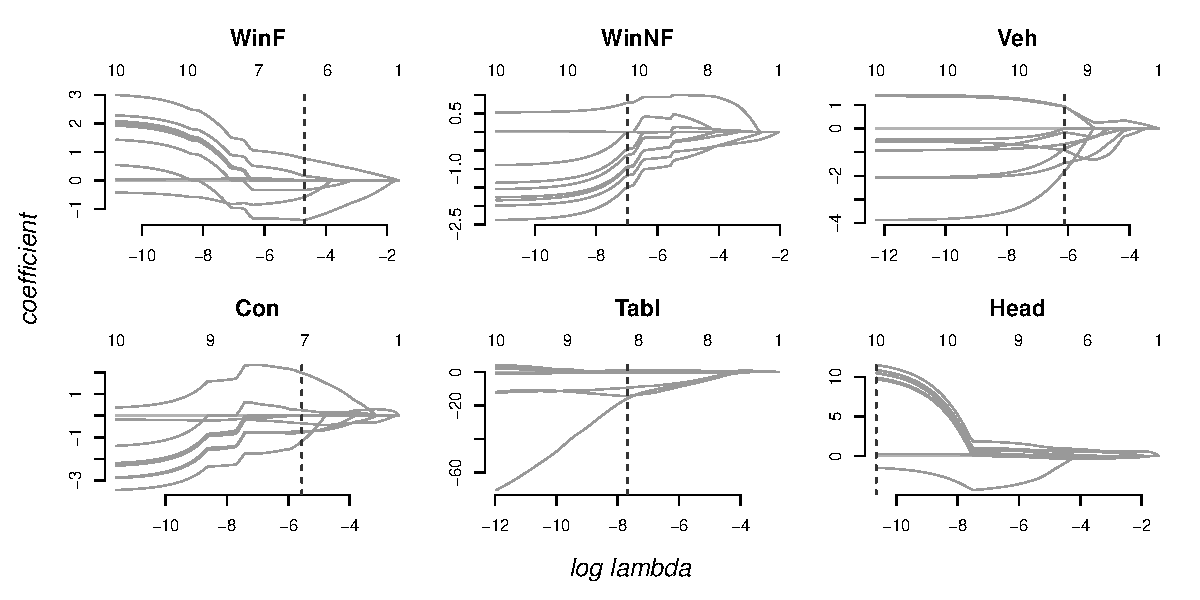
\includegraphics[width=6.25in]{fgl_coef}
\caption{\label{fgl_coef} {\it Forensic Glass}. Regularization paths for each glass-type, with AICc selections marked.}
\end{figure}


\begin{figure}
\begin{center}
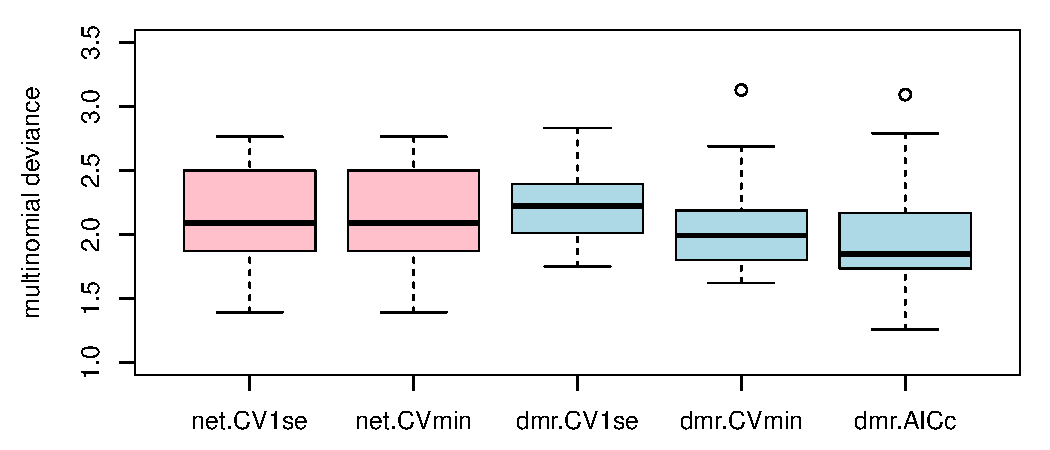
\includegraphics[width=5.75in]{fgl_cv}
\end{center}
\vskip -.5cm
\caption{\label{fgl_cv}  {\it Forensic Glass}. OOS deviance samples for \cd{dmr} and \cd{glment} in a 20-fold OOS experiment.  }\end{figure}



The response here is a single category, such that $m_i = 1$ and
$\hat\mu_i=0$ for all $i$.  This clearly violates the assumption of Poisson
generation: $m_i=1$ is not random.  For example, Figure \ref{fgl_mu} shows the conditional MLE $\mu_i^\star = \log\left(m_i/\sum_j e^{\hat\alpha_j + \bm{v}_i'\bs{\hat\varphi}_j}\right)$ at AICc selected coefficients.  The result is distributed around, but not equal to, the assumed plug-in of $\hat\mu_i=0$ for all $i$.  However \cd{dmr} still works:  Figure \ref{fgl_cv} 
shows the distribution for OOS error in a 20-fold OOS experiment, either using AICc or CV selection {\it on each individual Poisson
regression}, against CV selected models from a lasso path for full
multinomial logistic regression as implemented in the \cd{glmnet} package for
\cd{R} \citep{friedman_regularization_2010}. There are subtle differences (e.g., AICc DMR selection has lower mean deviance with higher variance), but the full multinomial fits (\cd{glmnet}) do not have any clear advantage over the nearly $d$-times faster  approximation (\cd{distrom}).


\begin{figure}[h]\vskip .5cm
\hskip 4cm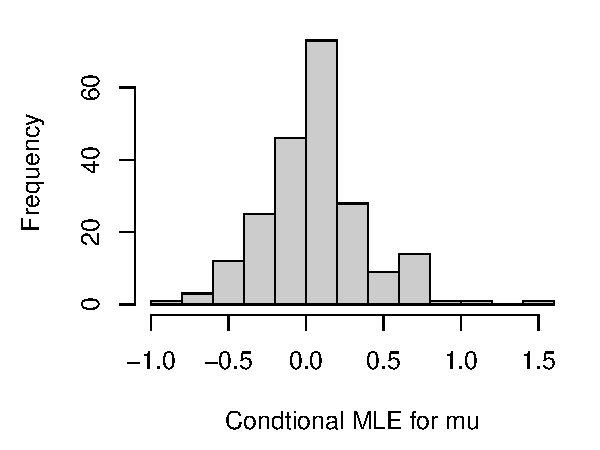
\includegraphics[width=3.25in]{fgl_mu}
\caption{\label{fgl_mu} {\it Forensic Glass}.  The  conditional MLEs $\mu^\star_i$ implied at our DMR coefficient estimates.   }
\vskip -.25cm
\end{figure}


\section{Yelp case study}
\label{YELP}


These data were supplied by the review site Yelp for a data mining contest on
\cd{kaggle.com}.  The data are available at
\cd{www.kaggle.com/c/yelp\!-\!recruiting/data}, and code for processing
and estimation is  at
\cd{github.com/TaddyLab/yelp}.  We consider business, user, and review datasets
in the \cd{yelp\_training\_data} collection.  The reviews, for all sorts of
businesses, were recorded on January 19, 2013 for a sample of locations near to
Phoenix AZ.  The goal of the competition was to predict the combined number of
`funny', `useful', or `cool' (f/u/c) votes that a given review receives from
other users.  Such information can be used by yelp to promote f/u/c  reviews
before waiting for the users to grade them as such.


After detailing the  data and model in Section
\ref{YELP}.1, we describe a series of statistical analyses.
\begin{itemize}\sgl
\item[\ref{YELP}.2] Investigate model fit under a range of regularization
schemes, looking at how word loadings change with the relative  weight of
penalty on variables of interest vs controls.
\item[\ref{YELP}.3] Use the ideas of `sufficient reduction' to project text
through the model onto topics relevant to f/u/c votes or star ratings, and
interpret the resulting factor spaces.
\item[\ref{YELP}.4] Apply these factor projections in prediction for the
number of f/u/c votes (i.e., the original \cd{kaggle} task), and compare
results against a standard lasso in OOS experimentation.
\item[\ref{YELP}.5] Use the factor projections in treatment effect
estimation -- for the effect of user experience on rating -- where they serve
to control for heterogenaity in review content.
\end{itemize}
By viewing text data as a big multinomial regression, we are able to address
all of the above (and resolve the effects of many collinear attributes on
review text) through a single model fit.

\subsection{Data and model specification}

The data are $n=$ 215,879 reviews on 11,535 businesses by 43,873
users.\footnote{We've removed reviews with unknown user} Review text is split
on whitespace and tokenized into words (including combinations of punctuation:
potential emoticons). After stripping some common suffixes (e.g., `s', `ing',
`ly') and removing a very small set of stopwords (e.g., `the', `and', `or'),
we count frequencies for $d=$ 13,938 words occurring in more than 20 ($<
0.01\%$) of the reviews (total word count is $M=$ 17,581,214).  

\begin{samepage}
\noindent Metadata
includes review, business, and user attributes.
\begin{itemize}\sgl
\item \cd{stars}: review star rating (out of 5), from which we subtract the business average rating.
\item Review counts for \cd{funny}, \cd{useful}, or \cd{cool} votes.  We divide these by the square root of review age, which yields metrics roughly uncorrelated with the posting date.
\item \cd{usr.count}: a user's total number of reviews at time of posting the given review
\item \cd{usr.stars}: a user's average star rating across all of their reviews.
\item A user's average \cd{usr.funny}, \cd{usr.useful}, or \cd{usr.cool} votes
per review.
\item Business average star rating \cd{biz.stars} and review count \cd{biz.count}.
\item Business location amongst 61 possible cities surrounding (and including) Phoenix.
\item Business classification according to Yelp's non-exclusive (and partially user generated) taxonomy.  We track membership  for 
333 categories  containing more than 5 businesses. 
\end{itemize}\end{samepage}
This yields 405 variables for each review.  We also specify random effects for
each of the 11,535  businesses, leading to total attribute dimension
$p=$ 11,940. Data components are the $n \times d$ document-term matrix $\bm{C}$, the
$n$-vector of its row-totals  $\bm{m}$, and the $n\times p$ attribute matrix
$\bm{V}$.  

We split each row of the attribute matrix into two elements: $\bm{a}_i$, the
11 numeric review attributes from \cd{stars} through
 \cd{biz.count}, and $\bm{b}_i$, a length-11,929 vector of dummy indicators for  business identity,
 location, and yelp classification.    This is done to differentiate the
 variables we deem of primary interest ($\bm{a}_i$) from those which we
 include as controls ($\bm{b}_i$); write $\bm{V} = [~\bm{A}~ \bm{B}~]$ as the
 resulting partition. Columns of $\bm{A}$ are normalized to have mean zero and
 variance one.  The multinomial regression  of (\ref{bigmn}) is adapted by
 similarly splitting each $\bs{\varphi}_j = [ {\bs{\varphi}_j^a},
 {\bs{\varphi}_j^b}]$ and rewriting category intensities
$
\log \lambda_{ij} = \alpha_j + \bm{a}_i'\bs{\varphi}^a_j + \bm{b}_i'\bs{\varphi}^b_j.
$

\subsection{Multinomial model fit and interpretation}

Following the recipe of Section \ref{GL}, 
each word's Poisson regression is estimated 
\begin{equation}\label{yelpobj}
 \hat\alpha_j,\bs{\hat\varphi}_j = 
 \argmin_{\alpha_j,\bs{\varphi}_j} \left\{l(\alpha_j,\bs{\varphi}_j) + n \lambda \left[\sum_k \omega^a_{jk} |\varphi^a_{jk} | + \frac{1}{\tau}\sum_k \omega^b_{jk} |\varphi^b_{jk} |\right]\right\},
\end{equation}
where $l(\alpha_j, \bs{\varphi}_j) = \sum_{i=1}^n \left[ m_i e^{\alpha_j +
\bm{a}_i'\bs{\varphi}_j^a+ \bm{b}_i'\bs{\varphi}_j^b} - c_{ij}(\alpha_j +
\bm{a}_i'\bs{\varphi}_j^a+ \bm{b}_i'\bs{\varphi}_j^b)\right]$.
The {\it relative penalty weight} $\tau > 0$ controls differential
regularization between the target variables and the controls. At larger $\tau$
values, there is less penalty on $\bs{\varphi}_j^b$ and the effect of
$\bm{b}_i$ on $c_{ij}$ has less opportunity to pollute our estimate for
$\bs{\varphi}_j^a$. That is, $\bs{\hat\varphi}_j^a$ becomes more purely a {\it
partial effect}. At the extreme of $\tau = \infty$, any collinearity with
$\bm{b}_i$ is be completely removed from the estimated $\bs{\hat\varphi}_j^a$.

As outlined in Appendix \ref{MR}, counts for the $14k$ words are partitioned
into 256 files.  Each file is then read by one of 64 workstations, which
itself uses 16 cores in parallel to run through the Poisson regressions. Each
individual regression is a full gamma lasso path solution over grids of 100
$\lambda_t$ squelch values, with weights $\omega_{jk}^{at},\omega_{jk}^{bt}$
updated as in (\ref{glweight}) under $\gamma=1$, and AICc selected
coefficients are then written to file. The entire problem (including the
sufficient reduction projection of our next section) takes around 1/2 hour.


\begin{figure}[b!]
\hspace{-.25in}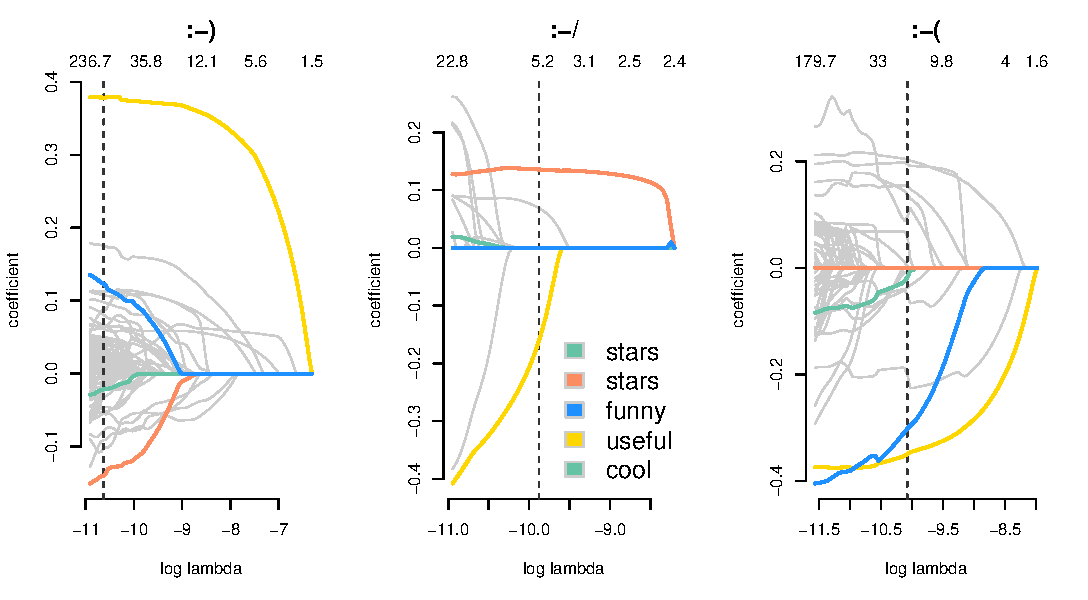
\includegraphics[width=6.75in]{yelp_ir_paths}
\caption{\label{yelp_ir} {\it Yelp}.  
Poisson regression regularization paths for counts of the tokens \cd{:-)},
\cd{:-/}, and
\cd{:-(} under relative penalty weight $\tau=2$.  Coefficient values have been
multiplied by the corresponding covariate standard deviation.  The legend
highlights select covariates, regression degrees of freedom are on the top
axis, and our AICc selected estimates are marked with vertical dashed lines. }
\end{figure}


Regularization paths for a few of the Poisson regressions, estimated under
$\tau=2$ relative penalty weight, are shown in Figure \ref{yelp_ir}.
Coefficient values are scaled to the effect of 1sd change in
the corresponding attribute. We see, for example, that at our AICc selection
the effect of a 1sd increase in review stars multiplies the expected count (or
odds, in the multinomial model) for the happy face
  \cd{:\!-\!)} by around $\exp 0.38 \approx 1.46$, the `hmmm' face \cd{:\!-\!/} by $\exp
  -0.15 \approx 0.86$, and the sad face \cd{:\!-\!(} by $\exp -0.35 \approx 0.7$.
 Notice that \cd{:\!-\!/} and \cd{:\!-\!(} both occur more often in low star
 (negative) reviews, but that \cd{:\!-\!/} is associated with useful content while
 \cd{:\!-\!(} is uncool.


Table \ref{topwords} investigates fit under increasing $\tau$, which allocates
more  count variation to the controls in $\bm{B}$.  The numbers of nonzero
$\hat\varphi^a_{jk}$  (i.e., deemed useful for OOS prediction by AICc) are
decreasing with $\tau$ for all attributes.  This is because $\bm{B}$ accounts
for more variation in $\bm{C}$ at higher $\tau$, and  there is little residual
variation left for $\bm{A}$.  At $\tau=200$, for example, there are only 7
words positively associated with a
\cd{cool} vote. Such differential penalization is a powerful tool in Big data
analysis,  as it allows one to isolate partial effects in messy overdetermined
systems.  Here, $\tau=2$ yields top words only indirectly
associated with our attributes (e.g., {\it prik} is positive because Thai food
is tasty), while  full $\tau=\infty$ control leads to near perfect fit and
infinite likelihoods conditional on $\bm{B}$ alone. To our eye, $\tau=20$
manages a good balance: there remain many significant
$\hat\varphi^a_{jk}\neq 0$, but the model has avoided loading  words that
are not directly associated with the given attributes.  This fit is used in
the remainder of our study.

\begin{table}[b!]
\footnotesize\setstretch{1.25}
\hspace{-.4cm}
\begin{tabular}{cll|r}
& \small $\bs{\tau}$ & \small $\bs{\hat\varphi \neq 0}$ 
& \small {\bf top ten words by loading}\\
\noalign{\smallskip}
\hline
 & \multicolumn{2}{l|}{marginal}    & \footnotesize\it great love amaz favorite deliciou best awesome alway perfect excellent \\
\small +stars & 2 & 8440 & \footnotesize\it  unmatch salute :-)) prik laurie pheonix trove banoffee exquisite sublime \\
 & 20 & 3077 & \footnotesize\it  heaven perfection gem divine amaz die superb phenomenal fantastic deliciousnes \\
 & 200 & 508 & \footnotesize\it  gem heaven awesome wonderful amaz fantastic favorite love notch fabulou \\
\hline
 &  \multicolumn{2}{l|}{marginal}   & \footnotesize\it  not worst ask horrib minut rude said told would didn \\
\small -stars & 2 & 8440 & \footnotesize\it  rude livid disrespect disgrace inexcusab grossest incompet audacity unmelt acknowledge \\
 & 20 & 3077 & \footnotesize\it  rude incompet unaccept unprofession inedib worst apolog disrespect insult acknowledge \\
 & 200 & 508 & \footnotesize\it  worst horrib awful rude inedib terrib worse tasteles disgust waste \\
\hline
 & \multicolumn{2}{l|}{marginal}   & \footnotesize\it  you that know like your yelp ... what don who \\
\small funny & 2 & 6508 & \footnotesize\it  dimsum rue reggae acne meathead roid bong crotch peni fart \\
 & 20 & 1785 & \footnotesize\it  bitch shit god dude boob idiot fuck hell drunk laugh \\
 & 200 & 120 & \footnotesize\it  bitch dear god hell face shit hipst dude man kidd \\
\hline
 &  \multicolumn{2}{l|}{marginal}   & \footnotesize\it  that yelp you thi know biz-photo like all http :// \\
\small useful & 2 & 5230 & \footnotesize\it  fiancee rife dimsum maitre jpg poultry harissa bureau redirect breakdown \\
 & 20 & 884 & \footnotesize\it  biz-photo meow harissa www bookmark :-/ http :// (?), tip \\
 & 200 & 33 & \footnotesize\it  www http :// com factor already final immediate ask hope \\
\hline
 &  \multicolumn{2}{l|}{marginal}   & \footnotesize\it  yelp you that biz-photo http :// www know like your \\
\small cool & 2 & 4031 & \footnotesize\it  boulder lewi rogue lagunita wanton celebratory hanker politic mozzerella onsite \\
 & 20 & 577 & \footnotesize\it  userid htm cen rand poem sultry arlin brimm cubic inspiration \\
 & 200 & 11 & \footnotesize\it  biz-photo select yelp along certain fil chose house  \\
\hline\end{tabular}
\caption[l]{\label{topwords}
Top 10 words by loading on review characteristics, as a function of relative
penalty weight $\tau$.  The top row for each attribute  corresponds to terms ordered by
marginal correlations.}
\end{table}


\subsection{Sufficient reduction}

The previous section's coefficient estimates, resolving a complex system of
 relationships between words and attributes,  provide a rich basis for
story telling and exploratory analysis. For many, this is either the end-goal
or a jumping-off point (e.g., to experiments testing hypotheses generated
in exploration).  But in our practice, a primary reason for fitting big
multinomial models is as a tool for {\it dimension reduction}, mapping from
the original $d$-dimensional text down to univariate indices that contain all
information relevant to a given attribute.  

\cite{cook_fisher_2007} outlines use of regression models with
high-dimensional response as a map to project from that response onto
interesting covariates.   \cite{taddy_multinomial_2013} extends the idea in
our context of big multinomials, motivated by applications in text analysis.
Both of these articles are focused on {\it inverse regression} (IR), a
technique wherein the fitted model map is applied for prediction of unobserved
covariates (e.g., the votes associated with new review text, as in Section
\ref{YELP}.4).  However, the IR algorithms are prefaced on a more basic
concept of {\it sufficient reduction} (SR), which is useful beyond its
application in IR prediction.

Consider observation $\bm{c}_i$ from a $d$ dimensional exponential family
linear model, with natural parameter $\bs{\eta}_i = [\eta_{i1} \ldots
\eta_d]'$,  $\eta_{ij} = \alpha_j + \bm{v}_i\bs{\varphi}_j$, such that
\begin{equation}\label{nef}
\mr{p}(\bm{c}_i) = h(\bm{c}_i)\exp\left[\bm{c}_i'\bs{\eta}_i + A(\bs{\eta}_i)\right]
\end{equation}
where $h$ is a function of only data (not $\bs{\eta}_i$) while $A$ is a
function of only parameters (not $\bm{c}_i)$.  Both the full
multinomial logistic regression model (conditional upon $m_i$) or our
independent Poissons model (conditional upon $\hat\mu_i$) can be written as in
(\ref{nef}). Then with $\bs{\Phi} = [\bs{\varphi}_1 \cdots
\bs{\varphi}_d]$ the $p\times d$ matrix of regression coefficients, we get
\begin{equation}\label{srproof}
\mr{p}(\bm{c}_i) = h(\bm{c}_i)e^{\bm{c}_i'\bs{\alpha}}
\exp\left[\bm{c}_i'\bs{\Phi}'\bm{v}_i + A(\bs{\Phi}'\bm{v}_i)\right] = 
\tilde h(\bm{c}_i)g(\bs{\Phi}\bm{c}_i,\bm{v}_i),
\end{equation}
so that the likelihood factorizes into a function of $\bm{c}_i$ only and
another function of $\bm{v}_i$ that depends upon $\bm{c}_i$ only through the
projection $\bs{\Phi}\bm{c}_i$.  This implies that, conditional upon
the regression parameters,  $\bs{\Phi}\bm{c}_i$ is a {\it
sufficient statistic} for $\bm{v}_i$.  That is, $\bm{v}_i \indep \bm{c}_i \mid
\bs{\Phi}\bm{c}_i$.

We call $\bm{z}_i = \bs{\Phi}\bm{c}_i$ an SR {\it projection}. In practice, we
work with estimated SR projections $\bm{z}_i =  \bs{\hat\Phi}\bm{c}_i$ and
hope that $\bs{\hat\Phi}$ has been estimated well enough for $\bm{z}_i$ to be
a useful summary \citep[see][for discussion]{taddy_rejoinder:_2013}. In that
case, $\bm{\hat\Phi}$ provides a linear map from text into the $p$-dimensional
attribute space.  This works just like the {\it rotation} matrix from common
principal components analysis except that, instead of mapping into latent
factors,  $\bs{\Phi}$ projects into observed attributes. The resulting
$\bm{z}_i$ are model-based sufficient statistics, useful in the same roles
as a traditional sufficient statistic (like $\bar x$). For example, to predict
$v_{ik}$ from $\bm{c}_i$ we can work with  univariate $z_{ik}$ instead of the
$d$-dimensional original text. In general, SR projections are a simple way to
organize information in Big data systems.  When new text $\bm{c}_i$ arrives,
one need just feed it through $\bs{\Phi}$ to obtain $\bm{z}_i$ indices which
can be summarized, plotted, and analyzed as desired.


It is important to emphasize that, since  estimated loadings
$\hat\varphi_{ik}$ are partial effects (influence of other attributes has
been controlled for), $z_{ik}$ will also correspond to partial rather
than marginal association. As another way to see this, note that the
 factorization in (\ref{srproof}) is easily manipulated to show
sufficiency for each individual $z_{ik}$ conditional on $\bm{v}_{i,-k}$, our
vector of attributes ommiting the $k^{th}$.  Thus SR reduces
dimension into a space of information {\it directly} relevant to an attribute
of interest, where influence of text variation due to other 
attributes has been removed or minimized. Consider the correlation matrices in
Figure
\ref{zcor}.  The original vote attributes  are highly positively correlated,
while the text projections are either nearly independent (e.g., {\tt useful}
against either \cd{funny} or
\cd{cool}) or strongly negatively correlated (\cd{funny} and \cd{cool}).  This
suggests that there are underlying factors that encourage {\it votes in any
category}; only after controlling for these confounding factors do we see the
true association between f/u/c content.  Similarly, all vote attributes are
uncorrelated with star rating, but for the text projections we see both negative
(\cd{funny},\cd{useful}) and positive (\cd{cool}) association.


\begin{figure}[htb]
\setstretch{1.1} \small 
\vskip .25cm
{\bf Correlation matrices}

\begin{center}
~~~~~~\begin{tabular}{r|ccccr|cccc}
 \multicolumn{4}{l}{\it attributes ($\bm{v}$)} & & 
 \multicolumn{4}{l}{\it \hskip 2cm text projections ($\bm{z}$)} \\ 
 %\multicolumn{10}{c}{}\\
\multicolumn{1}{c}{}& f & u &c & $\star$ &  \multicolumn{1}{c}{}&f & u &c & $\star$\\
\cline{2-5}\cline{7-10}
funny &  1 &  0.7 &  0.8 &   0 & \hskip 2cm funny &  1 &  -0.1 &  -0.7 &  -0.4\\
useful &  0.7 &  1 &  0.9 &   0 & \hskip 2cm useful &  -0.1 &  1 &  0.1 &  -0.2\\
cool &  0.8 &  0.9 &  1 &   0 & \hskip 2cm cool &  -0.7 &  0.1 &  1 &  0.5\\
stars &   0 &   0 &   0 &  1 & \hskip 2cm stars &  -0.4 &  -0.2 &  0.5 &  1\\
\end{tabular}
\end{center}
\caption{ \label{zcor} Correlation  for the original review attributes
in $\bm{v}$ (left) and for $\bm{z}$ (right) SR text projection. }
\end{figure}

The three 50-100 word reviews in Figure \ref{threerev} provide further
illustration.  A single review (bottom) of a historical site scores highest in
${\tt funny}$ and ${\tt useful}$  attributes (and also in ${\tt cool}$). The
review is neither dry nor useless, but we imagine its high vote count has been
influenced by other factors; e.g., the page is heavily viewed, or
people who read reviews of national parks are more likely to vote. In
contrast, read the two reviews identified through our machine-learned SR
projections as having the most funny or useful text content.  The funny
review, for a pizza restaurant, is a fictional comedic story. The useful
review contains a high proportion of business photos ({\it biz-photo}), which
the multinomial model has identified as directly useful.



\begin{figure}[p]
\begin{center}\small
\framebox[0.95\textwidth]{
\parbox{0.9\textwidth}{
\setstretch{1.2}

\vskip .5cm
{\bf Funniest 50-100 word review, by SR projection $\bs{z_{\tt funny}}$.}

\vskip .2cm
{\it Dear La Piazza al Forno: We need to talk. I don't quite know how to say this so I'm just going to come out with it. I've been seeing someone else. How long? About a year now. Am I in love? Yes. Was it you? It was. The day you decided to remove hoagies from your lunch menu, about a year ago, I'm sorry, but it really was you...and not me.  Hey... wait... put down that pizza peel... try to stay calm... please? [Olive oil container whizzing past head] Please! Stop throwing shit at me... everyone breaks up on social media these days... or haven't you heard?  Wow, what a Bitch!}

\vskip .5cm
{\bf Most useful 50-100 word review, by SR projection $\bs{z_{\tt useful}}$.}

\vskip .2cm
{\it  We found Sprouts shortly after moving to town.  There's a nice selection of Groceries \& Vitamins.  It's like a cheaper, smaller version of Whole Foods.
[biz-photo] [biz-photo] We shop here at least once a week.  I like their selection of Peppers....I like my spicy food! [biz-photo][biz-photo][biz-photo] Their freshly made Pizza isn't too bad either. [biz-photo] Overall, it's a nice shopping experience for all of us. Return Factor - 100\%}

\vskip .5cm
{\bf Funniest and most useful 50-100 word review, as voted by Yelp users\\ (votes normalized by square root of review age).}

\vskip .2cm{\it
I use to come down to Coolidge quite a bit and one of the cool things I use to do was come over here and visit the ruins.  A great piece of Arizona history!  Do you remember the Five C's?  Well, this is cotton country. The Park Rangers will tell you they don't really know how old the ruins are, but most guess at around 600 years plus.  But thanks to a forward thinking US Government, the ruins are now protected by a 70 foot high shelter.  Trust me, it comes in handy in July and August, the two months I seem to visit here most.  LOL.  I would also recommend a visit to the bookstore.  It stocks a variety of First Nation history, as well as info on the area.
  http://www.nps.gov/cagr/index.htm.  While you are in Coolidge, I would recommend the Gallopin' Goose for drinks or bar food, and Tag's for dinner.  Both are great!}
\vskip .5cm
}}
\end{center}
\caption{\label{threerev} Illustration of the information contained in sufficient projections
$\bm{z}$.  The top two reviews are those, amongst all where $m\in (50,100)$,
with highest SR projection scores into the {\tt funny} and {\tt useful}
attribute spaces.  For comparison, we also show the single 50-100 word review
with highest values for both $v_{\tt funny}$ and $v_{\tt useful}$ (recall that
these are vote totals per square root review age).  Note that, since variance
of $\bm{z}$ increases with $m$, high scoring reviews tend to be longer.  One
can also, as in
\cite{taddy_multinomial_2013}, divide the SR projections by document length and work with normalized $z/m$.
On this scale, the funniest review is `{\it Holy Mother of God}' and the most
useful review is `{\it Ask for Nick!}'.}
\end{figure}


\subsection{Inverse regression for prediction}


Multinomial-based SR projections were originally motivated by \cite{taddy_multinomial_2013} for their use in {\it multinomial inverse regression} \citep[MNIR; see also][]{taddy_measuring_2013}.  Say $v_{iy}$, some element of the attribute vector $\bm{v}_i$, is viewed as a `response' to be predicted for future realizations.  For example, in the original {\tt kaggle} Yelp contest the goal was to predict $v_{i,\tt funny}$, $v_{i,\tt useful}$, or $v_{i,\tt cool}$ -- the vote attributes.  In such applications, an MNIR routine would use the SR projection into $v_{iy}$, $z_{iy} = \sum_j \hat \varphi_{jy} c_{ij}$, to build a {\it forward regression} that predicts $v_{iy}$ from $z_{iy}$, $\bm{v}_{i,-y}$ (attributes ommiting $y$), and $m_i$.\footnote{The SR result that applies here is $v_{iy} \indep \bm{c}_i \mid z_{iy}, \bm{v}_{i,-y}, m_i$. Since sufficiency for $z_{iy}$ from the multinomial factorization is {\it conditional upon $m_i$}, these document totals need to be conditioned upon in forward regression.}  This $p+1$ dimensional regression replaces the $d+p-1$ dimensional one that would have been necessary to predict $v_{iy}$ from $\bm{v}_{i,-y}$ and $\bm{c}_{i}$, the original text counts.

Estimating an {\it inverse} regression in order to get at another
{\it forward} regression may seem a strange use of resources.  But there are a
variety of reasons to consider MNIR. Computationally, through either the
techniques of this article or the collapsing of
\cite{taddy_multinomial_2013}, the multinomial regression estimation can occur
in distribution on many independent machines. This is useful when the full
count matrix $\bm{C}$ is too big to fit in memory.
Another reason to use MNIR is for statistical efficiency when $d$ is big
relative to $n$.  Assuming a multinomial distribution for $\bm{c}_i \mid
\bm{v}_i$ introduces information into the estimation problem (a less generous
term is `bias').  In particular, it implies that each of the $M
= \sum_i m_i$ counts are independent observations, such that the sample size
for learning $\bs{\Phi}$ becomes $M$ rather than $n$.  That is, 
estimation variance decreases with the number of words rather than the number
of documents \cite[see][]{taddy_rejoinder:_2013}.


\begin{table}\setstretch{1.1}
\begin{center}\vskip -.25cm
\begin{tabular}{llc|ccc}
&\multicolumn{2}{c}{\it forward regression}&\multicolumn{3}{c}{\it average out-of-sample $R^2$}\\
& input variables & dimension & {\tt funny} & {\tt useful} & {\tt cool}\\
\cline{2-6}
standard lasso & non-vote attributes, $\bm{C}$ & 25,876 & 0.308 & 0.291 & 0.339\\
 MNIR + lasso & non-vote attributes, $\bm{z}$, $\bm{m}$ & 11,940 & 0.316 & 0.296 & 0.341
\end{tabular}
\end{center}
\vskip -.25cm
\caption[l]{\label{yelp_cv} {\it Yelp}.  Out-of-sample $R^2$ in prediction for vote attributes (normalized by root review age) in 5-fold CV.  The top row shows a standard lasso regression from the vote attribute onto text and all non-vote attributes, while the bottom row holds results for MNIR followed by lasso regression from the vote attribute onto review length ($m_i$), non-vote attributes, and the corresponding univariate SR projection. }
\end{table}



As an illustration, Table \ref{yelp_cv} shows results for prediction of
individual f/u/c vote attributes, both through MNIR with lasso forward regression
and for a standard lasso onto the full text counts.  That is, MNIR fits
$\ds{E}[v_{iy}] = \beta_0 +
[\bm{v}_{i,-{\text{f/u/c}}},m_i,z_{iy}]'\bs{\beta}$ while the comparator fits
$\ds{E}[v_{iy}] = \beta_0 + [\bm{v}_{i,-{\text{f/u/c}}},\bm{c}_i]'\bs{\beta}$,
where $\bm{v}_{i,-{\text{f/u/c}}}$  denotes all non-vote attributes.  For MNIR
each $\bs{\hat \Phi}$ (hence, $z_{iy}$) is also  estimated using only the
training sample, and  in both cases prediction rules were selected via AICc
minimization along the $L_1$ regularization path. We see  that
MNIR forward regression, replacing 13,938 covariates from $\bm{c}_i$ with just
the two numbers $z_{yi}$ and $m_i$, does not suffer against the full lasso
comparator (indeed, it is very slightly better in each case). Such performance
is  typical of what we've observed in application.\footnote{In
\cite{taddy_multinomial_2013}, the MNIR routines more significantly outperform
lasso comparators in OOS prediction. However, the datasets used in that paper
are both very small, with $M\gg n$. Thus our statistical efficiency argument
-- that for MNIR estimation variance decreases with $M$ instead of $n$ -- is
   working heavily in favor of MNIR. Here, even though $M > n$,  vocabulary
   size $d$ is smaller than $n$ and linear regression is already plenty
   efficient.} This is not evidence that the text counts do not matter: each
   full lasso estimates at least 4,000 terms having non-zero coefficients.
   Rather, the multinomial model is a good enough fit that the factorization
   results of (\ref{srproof}) apply and all relevant information is contained
   in the SR projection.\footnote{We have also found success applying
   nonlinear learning (e.g., trees) in forward regression after SR projection.
   Methods that are too expensive or unstable on the full text work nicely on
   the reduced dimension subspace.}


Note that the MNIR forward regression ignores projection from text onto any
other non-vote attributes. This is because those attributes are conditioned
upon in forward regression.  Indeed,
\cite{taddy_multinomial_2013,taddy_rejoinder:_2013} argue that, in prediction
for a single variable, you only need fit the multinomial dependence between
counts and that single variable.  This yields SR projection based on marginal
association, which can work as well as that based on partial
association for simple predictions. The benefit of fitting models for
high-dimensional $\bm{v}_i$ is that we are then able to interpret the resulting
partial effects and SR projections, as in Sections
\ref{YELP}.2-\ref{YELP}.3.  It is also useful in more structured prediction
settings, as in the next section.

\subsection{Confounder adjustment in treatment effect estimation}

In our final example, we illustrate use of SR projections as convenient low
dimensional {\it controls} in treatment effect estimation.  The task here has
a particular attribute, say $d$, whose effect on another, say $y$, you want to
estimate.  You want to know what will happen to $y$ if $d$ changes
independently from  the other attributes.  Unfortunately, everything is
collinear in the data and both $y$ and $d$ could be correlated to other
unobserved confounders.  Your best option is to estimate the treatment effect
-- that of $d$ on $y$ -- while controlling for observable potential
confounders.  In text analysis, this includes controlling for the text content
itself.


Consider estimating the effect of a user's experience -- the number of reviews
that they have written -- on their expected rating.  That is, are experienced
users more critical, perhaps because they've become more discerning?  Or do
they tend to give more positive reviews, perhaps because community norms
encourage a high average rating? It is hard to imagine getting firm evidence
in either direction without running a randomized trial -- we will always be
worried about the effect of an omitted confounder.  However, we can try our
best and condition on available information.    In particular, we can
condition on  content to ask the question: even given the same review
message, would an experienced user give more or less stars than a newbie?

The response attribute, $v_{iy}$, is  {\it star rating}. The treatment, $v_{id}$, is the log {\it number of reviews} by the author
(including the current review, so never less than one).  Results for
estimation of the effect of $v_{id}$ on $v_{iy}$, conditioning on different
control variables, are detailed in Table \ref{treats}.   A na\"ive estimate
for the effect of experience on rating, estimated through the marginal
regression $\ds{E}[v_{iy}] = \beta_0 +  v_{id}\gamma$, is a $\hat\gamma =
0.003$ increase in number of stars per extra unit log review count. Use
$\bm{v}_{i,-yd}$ to denote all other attributes.  Then an improved estimate of
the treatment effect is obtained by fitting $\ds{E}[v_{iy}] = \beta_0 +
v_{id}\gamma +
\bm{v}_{i,-yd}'\bs{\beta}$, which yields the much larger $\hat\gamma = 0.015$.

Finally, we'd like to control for $\bm{c}_i$, the review content summarized as word counts.  It would also be nice to control for content interacting with attributes since, e.g., positive content for a restaurant might imply a different star rating boost than it does for a bowling alley.
Unfortunately, interacting 13,938 dimensional $\bm{c}_i$ with the 333 business categories yields almost 4.7 million regression coefficients.  This is more controls than we have observations.  However, the SR projections offer a low-dimensional alternative.
Write $z_{iy}$ and $z_{id}$ for the SR
projections onto response and treatment, respectively.  Then sufficiency factorization implies
\begin{equation}
v_{iy},v_{id} \indep \bm{c}_i \mid z_{iy},z_{id},m_i,\bm{v}_{i,-yd}.
\end{equation}
That is,  the joint distribution of treatment and control is independent of
the text given SR projection into each.  This suggests we can control for
review content, and its interaction with business classification, simply by
adding to our conditioning set $[z_{iy},z_{id},m_i]$ and its interaction with
business classification. The resulting regression, with around 13$k$ control
coefficients instead of 4.7 million, yields the still larger treatment effect
estimate $\hat\gamma=0.02$.

\begin{table}[htb]\small
\vskip .25cm
\begin{tabular}{l|ccc}
& Marginal & Conditional on attributes only & Adding and interacting text SR \\
\cline{2-4}
Effect estimate & 0.003 & 0.015 & 0.020
\end{tabular}
\caption{\label{treats} Estimated effect `$\gamma$' of user experience (log
number of reviews) on number of stars rated.  Each corresponds to different
levels of confounder adjustment.  The effects are all AICc selected estimates
along a $\gamma=10$ (very near to $L_0$) gamma lasso regularization path,
where {\it all of the other regression coefficients} were unpenalized. Thus
they are significant, in the sense that the AICc deems $v_{id}$ useful for
predicting $v_{iy}$ even after all variation explained by confounders has been
removed.}
\end{table}


\section{Discussion}
\label{END}

Distributed estimation for multinomial regression allows such models to be applied on a new  scale, one that is limited only by the
number of machines you are able to procure. This advance is important for applied
work.  The collapsing of
\cite{taddy_multinomial_2013} is useful in prediction problems, but today
we more often find ourselves addressing inference and interpretation.  High dimensional
attribute sets are essential for such problems because multinomial model needs
to believable. This is in contrast to pure prediction problems where, as
outlined in \cite{taddy_rejoinder:_2013}, one can model inverse regression
misspecification during forward regression.

One message of this paper has been that Poisson factorization
enables fast estimation of multinomial distributions.  It has been pointed out
to us that, in unstructured data analysis, a Poisson seems little more
arbitrary than a multinomial model.  Equation (\ref{embed}) clarifies this
issue:  the only additional assumption one makes by working with independent
Poissons is that the aggregate total, $m_i$, is Poisson.  We've attempted to
mitigate the influence of this assumption, but that is unnecessary if you
consider the Poisson a fine model in and of itself.

\appendix
\section{Appendix}

\subsection{MapReduce} 
\label{MR}

  MapReduce \citep[MR;][]{dean_mapreduce:_2004} is a  recipe
for analysis of massive datasets, designed to work when the data itself is
distributed: stored in many files on a network of distinct machines.
The most common platform for  MR is Hadoop paired with a distributed file-
system (DFS)  optimized for such operations (e.g., Hadoop DFS or
Amazon's S3 storage).

A MapReduce routine has three main steps: map, partition, and reduce.  The
partition  is handled by Hadoop, such that we need worry only
about map and reduce.  The map operation parses  unstructured data into a
special format.  For us, in a text mining example, the mapper program will
take a document as input, parse the text into tokens (e.g. words), and output
lines of processed token counts: `\cd{token   document|count}'.  The pre-tab
item (our \cd{token}) is called a `key'.  Hadoop's sort facility uses these
keys to send the output of your mappers to machines for the next step,
reducers, ensuring that all instances of the same key (e.g., the same word)
are grouped together at a single reducer.  The reducer then executes some
operation that is independent-by-key, and the output is written to file
(usually one file per reducer).

DMR fits nicely in the MR framework.  Our map step tokenizes your unstructured data  and organizes the output by token keys.  Reduce then takes all observations on a single token and runs a Poisson log regression, applying the gamma lasso with IC selection to obtain coefficient estimates.  These are used to build our SR scores, which can be employed in forward regression after the MR routine is done.  This recipe is detailed in Algorithm \ref{mralgo}.

\begin{algorithm}[htb]
\caption{\label{mralgo} MapReduce DMR }
\vskip .25cm
{\bf Map:}  For each document, tokenize and count sums for each token.  Save the total counts $m_i$ along with attribute information $\bm{v}_i$. Output \cd{token   document|count}.

\vskip .25cm
Combine totals $m_i$ and attributes $\bm{v}_i$ into a single table, say \cd{VM}. This info can be generated during map or extracted in earlier steps.  Cache \cd{VM} so it is available to your reducers.

\vskip .25cm
{\bf Reduce:} For each token key `$j$', obtain a regularization path for Poisson regression of counts $c_{ij}$ on attributes $\bm{v}_i$ with $\hat\mu_i = \log m_i$.  Apply AICc to select a segment of coefficients from this path, say $\bs{\hat\varphi}_j$, and output nonzero elements in sparse triplet format: \cd{word|attribute|phi}. 

\vskip .25cm
Each reducer writes coefficients $\bs{\hat\varphi}_j$ of interest to file, and maintains a running total for SR projection, $\bm{z}_i +\!\!= \bm{c}_i'\bs{\hat \varphi_j}$, output as say \cd{Z.r} for the $r^{th}$ reducer.  When all machines are done we aggregate \cd{Z.r} 
to get the complete projections.  

~
\end{algorithm}



We've written this as a single MR algorithm, but other variations may work better for your computing architecture. Our most common implementation uses streaming Hadoop on Amazon Web Services (AWS) to execute the map on a large number of files in AWS S3 cloud storage, but replaces the regression reduce step with a simple write, to solid state storage `midway' at the University of Chicago's Research Computing Center, of token counts tabulated by observation.  For example, given 64 reducer machines on AWS the result is 64 text tables on midway, with lines `\cd{word|doc|count}', each containing {\it all} nonzero counts for a subset of the vocabulary of tokens.  These files are small enough to fit in working memory\footnote{If not, use more reducers or split the files.} and can be analyzed on distinct compute nodes, each employing another layer of parallelization in looping through Poisson regression for each token.  This scheme is able to take advantage of Hadoop for fast tokenization of distributed data, and of
high performance computing architecture (much faster than, say, a virtual AWS instance) for distributed  regression analyses.  This is a model that should work well for the many statisticians who have access to computing grids that are designed for high throughput tasks more traditionally associated with physics or chemistry.

\sgl\small
\bibliographystyle{asa}
\bibliography{dmr}


\end{document}
